\documentclass[12pt]{article}

% Imports the catppuccin theme, using the mocha flavor,
% from the directory above. Actual implementation
% wouldn't need the import package unless the theme
% and the document are in different directories.
\usepackage{import}
\usepackage{xcolor}
\usepackage{cancel}
\usepackage{mathtools}

\newcommand\Myperm[2][^n]{\prescript{#1\mkern-2.5mu}{}P_{#2}}
\newcommand\Mycomb[2]{\prescript{#1\mkern-0.5mu}{}C_{#2}}


\definecolor{yorhabg}{HTML}{1F1F1F}
\definecolor{yorhafg}{HTML}{CCCCCC}
\definecolor{yorhagrid}{HTML}{B5AF9C}
\definecolor{mred}{HTML}{F14C4C}
\definecolor{mblue}{HTML}{3BA3F0}

\pagecolor{yorhabg}
\color{yorhafg}

\import{/home/bhuv/Documents/ai_notes/code_stuff}{preamble.sty}

% Removes padding above title
\usepackage{titling}
\setlength{\droptitle}{-10em}

% Font package
\usepackage[T1]{fontenc}

\usepackage{fouriernc}

\usepackage{sectsty}
\usepackage{graphicx}
\usepackage{amsmath}
\usepackage{amsfonts}
\usepackage{amssymb}
\usepackage{tcolorbox}
\tcbuselibrary{listings, skins, breakable, most}

\DeclareMathOperator{\sgn}{sgn}

\usepackage{tikz}
\usepackage{eso-pic}
\usetikzlibrary{calc,shadows.blur}
\usetikzlibrary{angles, quotes}
\usetikzlibrary{3d}
\usetikzlibrary{positioning, arrows.meta}
\usepackage{listofitems} % for \readlist to create arrays
\usepackage[outline]{contour} % glow around text
\contourlength{1.4pt}

% \AddToShipoutPictureBG{%
% \begin{tikzpicture}[remember picture, overlay,
%                    help lines/.append style={line width=0.05pt, color=yorhagrid}]
%  \draw[help lines] (current page.south west) grid[step=5pt]
%                    (current page.north east);
% \end{tikzpicture}%
% }

% Margins
\topmargin=0in
\evensidemargin=0in
\oddsidemargin=0in
\textwidth=6.5in
\textheight=9.0in
\headsep=0.25in

\AtBeginEnvironment{tcolorbox}{\small}

\newtcolorbox{question}{%
    enhanced,
    colback=yorhabg,
    colframe=yorhafg,
    coltext=yorhafg,
    coltitle=yorhabg,
    title=\texttt{ooooo},
    arc=10pt,
    outer arc=10pt,
}

\newtcolorbox{imp}{enhanced,arc=0mm,colback=yorhabg,colframe=mred,leftrule=10mm,coltext=yorhafg,%
overlay={\node[anchor=west,outer sep=2pt] at (frame.west) {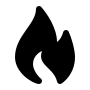
\includegraphics[width=6mm]{images/imagee.png}}; }}

\newtcolorbox{shortcut}{enhanced,arc=0mm,colback=yorhabg,colframe=mred,leftrule=10mm,coltext=yorhafg, coltitle=yorhabg, title=\texttt{Shortcut.}, 
overlay={\node[anchor=west,outer sep=2pt] at (frame.west) {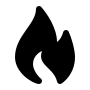
\includegraphics[width=6mm]{images/imagee.png}}; }}

\newtcolorbox{questionn}[1]{ % [1] = takes 1 argument
    enhanced,
    colback=yorhabg,
    colframe=mblue,
    coltext=yorhafg,
    coltitle=yorhabg,
    attach boxed title to top left={yshift*=-\tcboxedtitleheight}, 
    title=\texttt{#1}, % use the argument
    boxed title size=title,
    boxed title style={%
        rounded corners=northeast, 
        rounded corners=northwest, 
        colback=tcbcolframe, 
        boxrule=0pt,
    },
    underlay boxed title={%
        \path[fill=tcbcolframe] (title.south west)--(title.south east) 
            to[out=0, in=180] ([xshift=5mm]title.east)--
            (title.center-|frame.east)
            [rounded corners=5pt] |- 
            (frame.north) -| cycle; 
    },
}

\usepackage{xcolor}
\colorlet{myred}{red!80!black}
\colorlet{myblue}{blue!80!black}
\colorlet{mygreen}{green!60!black}
\colorlet{myorange}{orange!70!red!60!black}
\colorlet{mydarkred}{red!30!black}
\colorlet{mydarkblue}{blue!40!black}
\colorlet{mydarkgreen}{green!30!black}

\lstset{
  language=Python,
  frame=single,
  numbers=left,
  numberstyle=\tiny\color{gray!70},
  backgroundcolor=\color{black!90},
  basicstyle=\ttfamily\footnotesize\color{white!95},
  keywordstyle=\color{blue!70}\bfseries,
  stringstyle=\color{orange!80},
  commentstyle=\color{green!50}\itshape,
  identifierstyle=\color{white!90},
  emphstyle=\color{yellow!85}\bfseries,
  showstringspaces=false,
  tabsize=4,
  breaklines=true,
  captionpos=b,
  frameround=tttt,
  rulecolor=\color{gray!20}
}

% mac_vscode_lstset.tex
% Usage: compile with pdflatex/xelatex (no special engine required).
% This file defines a `macvscode` listings style and a `maclisting` environment
% that renders code inside a mac-like window (three buttons on top) and
% a Visual Studio Code-like dark color scheme

% Packages


% ---------------------------
% Color palette (VS Code-ish)
% ---------------------------

\definecolor{vscode-bg}{HTML}{1E1E2E} % editor background
\definecolor{vscode-line}{HTML}{2A2A33} % slightly lighter bg for code area
\definecolor{vscode-text}{HTML}{D4D4D4} % default text
\definecolor{vscode-comment}{HTML}{6A9955} % comments (green)
\definecolor{vscode-keyword}{HTML}{569CD6} % keywords (blue)
\definecolor{vscode-func}{HTML}{DCDCAA} % function names (yellowish)
\definecolor{vscode-string}{HTML}{CE9178} % strings (orange)
\definecolor{vscode-number}{HTML}{B5CEA8} % numbers
\definecolor{vscode-line-num}{HTML}{858585}% line numbers
\definecolor{mac-red}{HTML}{FF5F56}
\definecolor{mac-yellow}{HTML}{FFBD2E}
\definecolor{mac-green}{HTML}{27C93F}


% ---------------------------
% listings style
% ---------------------------
\lstdefinestyle{macvscode}{
backgroundcolor=\color{vscode-bg},
basicstyle=\ttfamily\small\color{vscode-text},
keywordstyle=\color{vscode-keyword}\bfseries,
commentstyle=\color{vscode-comment}\itshape,
stringstyle=\color{vscode-string},
numberstyle=\scriptsize\color{vscode-line-num},
showstringspaces=false,
breaklines=true,
frame=none,
tabsize=2,
emphstyle=\color{vscode-func},
columns=fullflexible,
}


% ---------------------------
% mac-like tcolorbox with rounded corners & stronger borders
% ---------------------------
\newtcblisting{maclisting}[2][]{%
enhanced,
breakable,
arc=6pt, % rounded corners
colback=vscode-bg,
colframe=vscode-line,
boxrule=1pt,
listing only,
listing options={style=macvscode,#1},
top=22pt,
overlay={%
\begin{scope}[shift={(frame.north west)}]
% top bar rectangle with rounded top corners
\path[fill=vscode-line,rounded corners=6pt] (0,0) rectangle (\linewidth,-20pt);
% three mac buttons
\fill[mac-red] (12pt,-10pt) circle (4pt);
\fill[mac-yellow] (28pt,-10pt) circle (4pt);
\fill[mac-green] (44pt,-10pt) circle (4pt);
% filename centered higher (closer to top bar)
\node[anchor=center] at (\linewidth/2,-10pt) {\small\color{vscode-text}#2};
\end{scope}
},
}


% STYLES
\tikzset{
  >=latex, % for default LaTeX arrow head
  node/.style={thick,circle,draw=myblue,minimum size=22,inner sep=0.5,outer sep=0.6},
  node in/.style={node,green!20!black,draw=mygreen!30!black,fill=mygreen!25},
  node hidden/.style={node,blue!20!black,draw=myblue!30!black,fill=myblue!20},
  node convol/.style={node,orange!20!black,draw=myorange!30!black,fill=myorange!20},
  node out/.style={node,red!20!black,draw=myred!30!black,fill=myred!20},
  connect/.style={thick,mydarkblue}, %,line cap=round
  connect arrow/.style={-{Latex[length=4,width=3.5]},thick,mydarkblue,shorten <=0.5,shorten >=1},
  node 1/.style={node in}, % node styles, numbered for easy mapping with \nstyle
  node 2/.style={node hidden},
  node 3/.style={node out}
}
\def\nstyle{int(\lay<\Nnodlen?min(2,\lay):3)}

\newcommand\bb[1]{\textcolor{yorhafg}{\textbf{#1}}}

\title{\textbf{Neural Networks \& Deep Learning}}
\author{ Bhuv }
\date{\today}

\begin{document}

\maketitle    

\section*{Linear Neural Network. (Simple)}

We never use Linear Neural Networks (1 input, 1 hidden layer, 1 output). Usually we use multiple inputs and multiples hidden layers. This is just for understanding. So, let's consider a simple example.

\begin{center}
\begin{tikzpicture}[>=Stealth, every node/.style={font=\small}, node distance=20mm]

  % nodes
  \node[draw,circle,minimum size=9mm] (x) {$x$};
  \node[draw,circle,minimum size=9mm, right=of x] (h) {$h$};
  \node[draw,circle,minimum size=9mm, right=of h] (y) {$y$};

  % labels on top
  \node[above=3mm of x] {Input};
  \node[above=3mm of h] {Hidden (linear)};
  \node[above=3mm of y] {Output};

  % arrows & weight labels
  \draw[->] (x) -- node[above, mred] {$w_1$} node[below, mblue]{\(b_1\) } (h);
  \draw[->] (h) -- node[above, mred] {$w_2$} node[below, mblue]{\(b_2\) }(y);

\end{tikzpicture}
\end{center}

\subsection*{Forward Propagation.}

So here, after the input, we have a linear transformation to the hidden layer. 

\[
    O_{x} = w_1 \cdot x + b_1
\]

This is the output after the linear transformation. We have to apply the activation function to introduce non-linearity to the learning. 

\[
    h = f_{a} (O_{x}) = f_{a} (w_1 \cdot x + b_1)
\]

And now the hidden layer undergoes the same process as the input layer. 

\[
    O_{h} = w_2 \cdot h + b_2
\]

And finally, we apply the activation function again to get the output.

\[
    y = f_{a} (O_{h}) = f_{a} (w_2 \cdot h + b_2)
\]

\vspace{0.1in}

\begin{imp}
    If we don't apply the activation function, the model will only learn linear relationships, limiting its capacity to capture complex patterns in the data. And also the activation function helps in normalizing the output, making it easier to handle and interpret. AND, the activation function is the same for every layer, we use only a single activation function for the entire network. 
\end{imp}

\vspace{0.1in}

We got the output, now what ? We check whether it is correct or not and then punish the model if it is wrong (which it will be, in the beginning stages of learning). How do we do that ??

We calculate the loss, which is a measure of how far the model's predictions are from the actual target values. The loss function quantifies this difference, and our goal is to minimize it during training.

\subsection*{Loss Function \& Gradient Descent.}

The most basic and wide-known loss function is the MSE Loss, which is just the mean squared error. Continuing from the previous equations, let's define the correct answer (label) as \(y_{\text{true} }\) and our predicted output as \(y_{\text{pred} } \) 

\[
    \Delta = \frac{1}{n} \sum_{i=1}^{n} (y_{\text{pred} }^i - y_{\text{true} }^i)^2
\]

Since we have only one output, 

\[
    \Delta =  (y_{\text{pred} } - y_{\text{true} })^2
\]

This is the Loss function, which we want to minimize to minimize the error in predictions. To minimize the loss, we use a technique called Gradient Descent. The idea is to compute the gradient (or derivative) of the loss function with respect to the model parameters (weights and biases) and then update the parameters in the opposite direction of the gradient.

The update rule for a parameter \( \theta  \) is given by:

\[
    \theta   = \theta   - \eta \cdot \frac{\partial \Delta}{\partial \theta}
\]

where \( \eta \) is the learning rate, a hyperparameter that controls how much we adjust the parameters at each step.

\subsection*{Backpropagation.}

How it works is that first we calculate the "gradient" (slope) of the function with respect to each weight and minimize the error w.r.t to that particular weight by changing the value of the weight towards the downhill of the slope, ultimately leading to a minimum. This happens for every single weight and bias in the network. For that, we need to find the gradient w.r.t to that particular parameter. We use chain rule to achieve that. 

\[
    \frac{\partial \Delta}{\partial w_2} = \frac{\partial \Delta }{\partial y_{\text{pred} } } \cdot  \frac{\partial y_{\text{pred} } }{\partial O_{h} } \cdot \frac{\partial O_{h}}{\partial w_2}
\]


Now, calculating the direct equations for the above gradient, 

\[
    \frac{\partial \Delta}{\partial w_2} = \frac{\partial \Delta }{\partial y_{\text{pred} } } \cdot  \frac{\partial y_{\text{pred} } }{\partial O_{h} } \cdot \frac{\partial O_{h}}{\partial w_2} = 2 (y_{\text{pred} } - y_{\text{true} }) \cdot f_{a} ^{\prime} (O_{h} ) \cdot h
\]

\vspace{0.1in}

\begin{questionn}{Sigmoid Activation function.}
    Here, lets take the Sigmoid activation function, which is defined as
    \[
    f_{a}(x) = \frac{1}{1 + e^{-x}}
    \]
    The derivative of the Sigmoid function is given by
    \[
    f_{a}^{\prime}(x) = f_{a}(x) \cdot (1 - f_{a}(x))
    \]
\end{questionn}

So, we get the final value as, 

\[
    \frac{\partial \Delta }{\partial w_2}  = 2 (y_{\text{pred}} - y_{\text{true} }) \cdot \frac{1}{1 + e^{O_{h} }} \cdot ( \frac{e^{-O_{h} } }{1 + e^{-O_{h} } }) \cdot h
\]

Now for the other weight, it'll be

\[
    \frac{\partial \Delta }{\partial w_1} = \frac{\partial \Delta }{\partial y_{\text{pred} } } \cdot  \frac{\partial y_{\text{pred} } }{\partial O_{h} } \cdot \frac{\partial O_{h}}{\partial h} \cdot \frac{\partial h}{\partial O_{x} } \cdot \frac{\partial O_{x}}{\partial w_1}
\]

You expand this and find the value of the gradient and apply gradient descent for the respective weights and change them. The same thing happens for biases. 

\vspace{0.2in}
\hrule

\section*{2-Dimensional Neural Network.}

In a 2-dimensional neural network, we have 2 inputs, 1 hidden layer (2 units) and 2 outputs. The architecture looks something like. 

\begin{center}
\begin{tikzpicture}[>=Stealth, every node/.style={font=\small}, node distance=20mm]

  % Input layer
  \node[draw,circle,minimum size=9mm] (x1) {$x_1$};
  \node[draw,circle,minimum size=9mm, below=of x1] (x2) {$x_2$};

  % Hidden layer
  \node[draw,circle,minimum size=9mm, right=40mm of x1] (h1) {$h_1$};
  \node[draw,circle,minimum size=9mm, below=of h1] (h2) {$h_2$};

  % Output layer
  \node[draw,circle,minimum size=9mm, right=40mm of h1] (y1) {$y_1$};
  \node[draw,circle,minimum size=9mm, below=of y1] (y2) {$y_2$};

  % Inputs → Hidden
  \draw[->] (x1) -- (h1)
    node[midway,above] {$w_{11} ^{(1)}$}
    node[midway,below] {$b_{11}^{(1)}$};
  \draw[->, mred] (x1) -- (h2)
    node[midway,above,xshift=-18pt, yshift=12pt] {$w_{21}^{(1)}$}
    node[midway,below,xshift=-18pt, yshift=12pt] {$b_{21}^{(1)}$};
  \draw[->, mblue] (x2) -- (h1)
    node[midway,above,xshift=18pt, yshift=12pt] {$w_{12}^{(1)}$}
    node[midway,below,xshift=18pt, yshift=12pt] {$b_{12}^{(1)}$};
  \draw[->] (x2) -- (h2)
    node[midway,above] {$w_{22}^{(1)}$}
    node[midway,below] {$b_{22}^{(1)}$};

  % Hidden → Output
  \draw[->] (h1) -- (y1)
    node[midway,above] {$w_{11}^{(2)}$}
    node[midway,below] {$b_{11}^{(2)}$};
  \draw[->, mred] (h1) -- (y2)
    node[midway,above,xshift=-18pt, yshift=12pt] {$w_{21}^{(2)}$}
    node[midway,below,xshift=-18pt, yshift=12pt] {$b_{21}^{(2)}$};
  \draw[->, mblue] (h2) -- (y1)
    node[midway,above,xshift=18pt, yshift=12pt] {$w_{12}^{(2)}$}
    node[midway,below,xshift=18pt, yshift=12pt] {$b_{12}^{(2)}$};
  \draw[->] (h2) -- (y2)
    node[midway,above] {$w_{22}^{(2)}$}
    node[midway,below] {$b_{22}^{(2)}$};

  % Labels on top of layers
  \node[above=3mm of x1] {Inputs};
  \node[above=3mm of h1] {Hidden layer};
  \node[above=3mm of y1] {Outputs};

\end{tikzpicture}
\end{center}

\subsection*{Forward Propagation.}

Here, the values of inputs are passed by multiplying with their weights and biases towards the neuron its going through next. For example, from \(x_1\) to \(h_1\), the output for \(x_1\) will be,

\[
    O_{x_1 \to h_1} = w_{11}^{(1)} \cdot x_1 + b_{11}^{(1)}
\]

But \(h_1\) also gets weighted value from \(x_2\) too. So, to simplify things, I'll be directly writing the final input for \(h_1\), including the activated function.

\[
    h_1 = \mathbf{A} (w_{11}^{(1)} \cdot x_1 + b_{11}^{(1)} + w_{12}^{(1)} \cdot x_2 + b_{12}^{(1)})
\]

Now, same thing happens for \(h_2\) too. So lets move on to the propagation from hidden layer to output layer. 

\[
  y_1 = \mathbf{A} (\underbrace{w_{11}^{(2)} \cdot h_1 + b_{11}^{(2)} + w_{12}^{(2)} \cdot h_2 + b_{12}^{(2)}}_{O_{y1} })
\]

\[
  y_2 = \mathbf{A} (\underbrace{w_{21}^{(2)} \cdot h_1 + b_{21}^{(2)} + w_{22}^{(2)} \cdot h_2 + b_{22}^{(2)}}_{O_{y2} })
\]

\subsection*{Gradient Descent \& Backpropagation.}

First, we calculate the loss function. We are gonna use MSE here. So, the equation is gonna be like

\[
  \Delta = \frac{1}{2} \sum_{i=1}^{2} (y_i - \hat{y}_i)^2
\]

You realise that despite summing them up, the gradients for each output are calculated independently during backpropagation because of partial derivatives. So, first we find the gradient of the loss function w.r.t \(w_{11}^{(2)} \).  

\[
  \frac{\partial \Delta }{\partial w_{11}^{(2)}} = \frac{\partial \Delta }{\partial y_1} \cdot \frac{\partial y_1}{\partial O_{y1} } \cdot \frac{\partial O_{y1} }{\partial w_{11}^{(2)}}
\]

Its very similar for the rest of the weights and biases that are from the hidden layer to the output layer. Things change when we want to find the gradient for the weights and biases from the input layer to the hidden layer. For calculating the gradient of the loss function w.r.t \(w_{11}^{(1)}\), we have to backpropagate via the two paths that are possible from the output layer to the first input. 

\begin{center}
\begin{tikzpicture}[>=Stealth, every node/.style={font=\small}, node distance=20mm]

  % Input layer
  \node[draw,circle,minimum size=9mm] (x1) {$x_1$};
  \node[draw,circle,minimum size=9mm, below=of x1] (x2) {$x_2$};

  % Hidden layer
  \node[draw,circle,minimum size=9mm, right=40mm of x1] (h1) {$h_1$};
  \node[draw,circle,minimum size=9mm, below=of h1] (h2) {$h_2$};

  % Output layer
  \node[draw,circle,minimum size=9mm, right=40mm of h1] (y1) {$y_1$};
  \node[draw,circle,minimum size=9mm, below=of y1] (y2) {$y_2$};

  % Inputs → Hidden
  \draw[->, mred] (x1) -- (h1);
  \draw[->] (x1) -- (h2);
  \draw[->] (x2) -- (h1);
  \draw[->] (x2) -- (h2);

  % Hidden → Output
  \draw[->, mred] (h1) -- (y1);
  \draw[->, mred] (h1) -- (y2);
  \draw[->] (h2) -- (y1);
  \draw[->] (h2) -- (y2);

  % Labels on top of layers
  \node[above=3mm of x1] {Inputs};
  \node[above=3mm of h1] {Hidden layer};
  \node[above=3mm of y1] {Outputs};

\end{tikzpicture}
\end{center}

So, the equation for the gradient w.r.t \(w_{11}^{(1)}\) is

\[
  \frac{\partial \Delta }{\partial w_{11}^{(1)}} = \frac{\partial \Delta }{\partial y_1} \cdot \frac{\partial y_1}{\partial O_{\textcolor{mblue}{y1}} } \cdot \frac{\partial O_{\textcolor{mblue}{y1}} }{\partial h_1} \cdot \frac{\partial h_1}{\partial O_{h1} } \cdot \frac{\partial O_{h1}}{\partial w_{11}^{(1)} } + \frac{\partial \Delta }{\partial y_2} \cdot \frac{\partial y_2}{\partial O_{\textcolor{mred}{y2}} } \cdot \frac{\partial O_{\textcolor{mred}{y2}} }{\partial h_1} \cdot \frac{\partial h_1}{\partial O_{h1} } \cdot \frac{\partial O_{h1}}{\partial w_{11}^{(1)} }   
\]

And its similar for \(w_{12}^{(1)}\).

\vspace*{0.2in}
\hrule

\section*{First Step Towards Generalization.}

We'll first generalize this for 2-D by making use of matrices and vectors. Then we'll generalize it for n-dimensions. Now, we'll introduce a new term \(\delta_i ^{(L)}\) where \(i\) is the index of the neuron in layer \(L\). 

\[
  \delta_1 ^{(3)} = \frac{\partial \Delta }{\partial y_1} \cdot \frac{\partial y_1}{\partial O_{y1} }  
\]

This is actually called the loss term of the neuron. This is quite useful in generlization. So basically, we can write 

\[
  \frac{\partial \Delta }{\partial w_{11}^{(2)}} = \delta_1 ^{(3)} \cdot \frac{\partial O_{y1} }{\partial w_{11}^{(2)}} = \delta_1 ^{(3)} \cdot h_1
\]

Now, we have 

\[
  \delta^{(3)} = \begin{bmatrix}
     \dfrac{\partial \Delta }{\partial y_1} \cdot \dfrac{\partial y_1}{\partial O_{y1} }   \\
     \\
     \dfrac{\partial \Delta }{\partial y_2} \cdot \dfrac{\partial y_2}{\partial O_{y2} }   \\
  \end{bmatrix} = \begin{bmatrix}
     \delta_1 ^{(3)} \\
     \\
     \delta_2 ^{(3)} \\
  \end{bmatrix}
\]

This is basically a vector of loss terms of the output layer. Now, we have the vector of outputs of the previous (hidden) layer as 

\[
  h = \begin{bmatrix}
    h_1 &  h_2 \\
  \end{bmatrix}
\]

Now, here's where the magic of matrices happens. The gradient of the weights from hidden layer to output layer can be represented as the multiplication of the loss term vector and the output vector of the previous layer. 

\[ 
  \dfrac{\partial \Delta }{\partial w_{ij}^{(2)} } = \begin{bmatrix}
     \delta_1 ^{(3)} \\
     \\
     \delta_2 ^{(3)} \\
  \end{bmatrix} \cdot \begin{bmatrix}
     h_1 &  h_2 \\
  \end{bmatrix} = \begin{bmatrix}
     \delta_1 ^{(3)} \cdot h_1 & \delta_1 ^{(3)} \cdot h_2 \\
     \\
     \delta_2 ^{(3)} \cdot h_1 & \delta_2 ^{(3)} \cdot h_2 \\
     \end{bmatrix}
\]

Now, we do the same for the weights from input layer to hidden layer. First, we find the loss term vector for the hidden layer. It can be defined in general terms as, 

\[
  \boxed{\delta_j ^{(l)} = \mathbf{A}^{\prime} (O_{h_j}) \cdot \sum_{i=1}^{l} \delta_i ^{(l+1)} \cdot w_{ij}^{(l)}}
\]

Don't worry if you don't understand this, it will be clear in a bit. So, for our case, we have our gradient as, 

\[
  \frac{\partial \Delta }{\partial w_{11}^{(1)}} = \frac{\partial \Delta }{\partial y_1} \cdot \frac{\partial y_1}{\partial O_{\textcolor{mblue}{y1}} } \cdot \frac{\partial O_{\textcolor{mblue}{y1}} }{\partial h_1} \cdot \frac{\partial h_1}{\partial O_{h1} } \cdot \frac{\partial O_{h1}}{\partial w_{11}^{(1)} } + \frac{\partial \Delta }{\partial y_2} \cdot \frac{\partial y_2}{\partial O_{\textcolor{mred}{y2}} } \cdot \frac{\partial O_{\textcolor{mred}{y2}} }{\partial h_1} \cdot \frac{\partial h_1}{\partial O_{h1} } \cdot \frac{\partial O_{h1}}{\partial w_{11}^{(1)} }   
\]

We are gonna simplify this. 

\[
  \dfrac{\partial \Delta }{\partial w_{11}^{(1)}} = \delta_1 ^{(3)} \cdot w_{11}^{(2)} \cdot \mathbf{A}^{\prime} (O_{h1}) \cdot \frac{\partial O_{h1}}{\partial w_{11}^{(1)}} + \delta_2 ^{(3)} \cdot w_{21}^{(2)} \cdot \mathbf{A}^{\prime} (O_{h1}) \cdot \frac{\partial O_{h1}}{\partial w_{11}^{(1)}}
\]

\[
  \dfrac{\partial \Delta }{\partial w_{11}^{(1)}} = \dfrac{\partial O_{h1} }{\partial w_{11} ^{(1)}} \cdot (\underbrace{\delta_1 ^{(3)} \cdot w_{11}^{(2)} \cdot \mathbf{A}^{\prime} (O_{h1} ) + \delta_2 ^{(3)} \cdot w_{21}^{(2)} \cdot \mathbf{A}^{\prime} (O_{h1} )}_{\delta_1 ^{(2)}})
\]

Now, if you go back and compare this with the definition, it matches perfectly. So, we have

\[
  \dfrac{\partial \Delta }{\partial w_{11}^{(1)}} = \delta_1 ^{(2)} \cdot (\dfrac{\partial O_{h1}  }{\partial w_{11}^{(1)}}) = \delta_1 ^{(2)} \cdot x_1
\]

So, now just like the previous layer, we can get the gradient matrix for the weights from input layer to hidden layer as

\[
  \dfrac{\partial \Delta }{\partial w_{ij}^{(1)} } = \begin{bmatrix}
     \delta_1 ^{(2)} \\
     \\
     \delta_2 ^{(2)} \\
  \end{bmatrix} \cdot \begin{bmatrix}
     x_1 &  x_2 \\
  \end{bmatrix} = \begin{bmatrix}
     \delta_1 ^{(2)} \cdot x_1 & \delta_1 ^{(2)} \cdot x_2 \\
     \\
     \delta_2 ^{(2)} \cdot x_1 & \delta_2 ^{(2)} \cdot x_2 \\
     \end{bmatrix}
\]

The process you see is generalizable to n-dimensions. Like, the same process repeats for subsequent hidden layers.

\vspace*{0.2in}
\hrule

\newpage

\section*{n-Dimensional Neural Network.}

\begin{center}
\begin{tikzpicture}[x=2.2cm,y=1.4cm]
  \message{^^JNeural network, shifted}
  \readlist\Nnod{4,5,5,5,3} % array of number of nodes per layer
  \readlist\Nstr{n,m,m,m,k} % array of string number of nodes per layer
  \readlist\Cstr{\strut x,a^{(\prev)},a^{(\prev)},a^{(\prev)},y} % array of coefficient symbol per layer
  \def\yshift{0.5} % shift last node for dots
  
  \message{^^J  Layer}
  \foreachitem \N \in \Nnod{ % loop over layers
    \def\lay{\Ncnt} % alias of index of current layer
    \pgfmathsetmacro\prev{int(\Ncnt-1)} % number of previous layer
    \message{\lay,}
    \foreach \i [evaluate={\c=int(\i==\N); \y=\N/2-\i-\c*\yshift;
                 \index=(\i<\N?int(\i):"\Nstr[\lay]");
                 \x=\lay; \n=\nstyle;}] in {1,...,\N}{ % loop over nodes
      % NODES
      \node[node \n] (N\lay-\i) at (\x,\y) {$\Cstr[\lay]_{\index}$};
      
      % CONNECTIONS
      \ifnum\lay>1 % connect to previous layer
        \foreach \j in {1,...,\Nnod[\prev]}{ % loop over nodes in previous layer
          \draw[connect,white,line width=1.2] (N\prev-\j) -- (N\lay-\i);
          \draw[connect] (N\prev-\j) -- (N\lay-\i);
          %\draw[connect] (N\prev-\j.0) -- (N\lay-\i.180); % connect to left
        }
      \fi % else: nothing to connect first layer
      
    }
    \path (N\lay-\N) --++ (0,1+\yshift) node[midway,scale=1.5] {$\vdots$};
  }
  
  % LABELS
  \node[above=1,align=center,mygreen!60!white] at (N1-1.90) {input\\[-0.2em]layer};
  \node[above=1,align=center,myblue!60!white] at (N3-1.90) {hidden layers};
  \node[above=1,align=center,myred!60!white] at (N\Nnodlen-1.90) {output\\[-0.2em]layer};
  
\end{tikzpicture}
\end{center}

\subsection*{Forward Propagation.}

Here, we have to use vectors to simplify the equations. So, the input for te first neuron in the first hidden layer will be, 

\[
  a_1 ^{(1)} = \sigma (\begin{bmatrix}
     x_1 \\
     \\
     x_2 \\
     \\
     x_3 \\
     \\
     \vdots \\
     \\
     x_n \\
  \end{bmatrix} \cdot \begin{bmatrix}
     w_{11}^{(1)} \\
     \\
     w_{12}^{(1)} \\
     \\
     w_{13}^{(1)} \\
     \\
     \vdots \\
     \\
     w_{n}^{(1)} \\
  \end{bmatrix} + \begin{bmatrix}
     b_1^{(1)} \\
     \\
     b_2^{(1)} \\
     \\
     b_3^{(1)} \\
     \\
     \vdots \\
     \\
     b_n^{(1)} \\
  \end{bmatrix} )
\]

Let's denote the vectors as a single letter (capital case) for simplicitiy. 

\[
  A^{(1)}= \sigma (\mathbf{X} \cdot \mathbf{W}^{(1)} + \mathbf{B}^{(1)})
\]

It repeats for the subsequent layers. So, for the output layer, 

\[
  \mathbf{Y} = \sigma (A^{(3)} \cdot \mathbf{W}^{(4)} + \mathbf{B}^{(4)})
\]


\newpage
\subsection*{Gradient Descent \& Backpropagation.}

Now, the Loss vector is

\[
  \mathbf{L}  = \frac{1}{n}(\mathbf{Y} - \hat{\mathbf{Y}}) ^2
\]

We can write the loss function as, 

\[
  \mathfrak{L} = \sum_{i=1}^{n} L_i, \quad \text{where } L_i \in \mathbf{L}
\]

Now, how does the backpropagation work here? There are so many weights and biases, how do we calculate the gradients for each of them? Look at what we did in the 2-D case. We defined a loss term for each neuron. We can do the same here. For the output layer, 

\[
  \delta_i ^{(4)} = \dfrac{\partial \mathfrak{L} }{\partial y_i} \cdot \dfrac{\partial y_{i} }{\partial O_{y_i} } 
\]

And so, we can write the loss term vector and previous layer output vector as the following and get the gradient matrix for the weights from hidden layer 3 to output layer as,

\[
  \dfrac{\partial \mathfrak{L} }{\partial w_{ij}^{(4)}} = \begin{bmatrix}
     \delta_1 ^{(4)} \\
     \\
     \delta_2 ^{(4)} \\
     \\
     \vdots\\
     \\
     \delta_n ^{(4)} \\
  \end{bmatrix} \cdot \begin{bmatrix}
     a_1 ^{(3)} &  a_2 ^{(3)} & \cdots & a_n ^{(3)} \\
  \end{bmatrix} = 
    \begin{bmatrix}
      \delta_1 ^{(4)} \cdot a_1 ^{(3)} & \delta_1 ^{(4)} \cdot a_2 ^{(3)}  & \cdots & \delta_1 ^{(4)} \cdot a_n ^{(3)} \\
      \\
      \delta_2 ^{(4)} \cdot a_1 ^{(3)} & \delta_2 ^{(4)} \cdot a_2 ^{(3)}  & \cdots & \delta_2 ^{(4)} \cdot a_n ^{(3)} \\
      \\
      \vdots & \vdots & \ddots & \vdots \\
      \\
      \delta_n ^{(4)} \cdot a_1 ^{(3)} & \delta_n ^{(4)} \cdot a_2 ^{(3)}  & \cdots & \delta_n ^{(4)} \cdot a_n ^{(3)} \\
    \end{bmatrix}
\]

The first row gives us the gradients of the weights going into the first neuron of the output layer. The second row gives us the gradients of the weights going into the second neuron of the output layer and so on. This can be generalized to any hidden layer as, 

\[
    \dfrac{\partial \mathfrak{L} }{\partial w_{ij}^{(L)}} = \begin{bmatrix}
     \delta_1 ^{(L)} \\
     \\
     \delta_2 ^{(L)} \\
     \\
     \vdots\\
     \\
     \delta_n ^{(L)} \\
  \end{bmatrix} \cdot \begin{bmatrix}
     a_1 ^{(L-1)} &  a_2 ^{(L-1)} & \cdots & a_n ^{(L-1)} \\
  \end{bmatrix} = 
    \begin{bmatrix}
      \delta_1 ^{(L)} \cdot a_1 ^{(L-1)} & \delta_1 ^{(L)} \cdot a_2 ^{(L-1)}  & \cdots & \delta_1 ^{(L)} \cdot a_n ^{(L-1)} \\
      \\
      \delta_2 ^{(L)} \cdot a_1 ^{(L-1)} & \delta_2 ^{(L)} \cdot a_2 ^{(L-1)}  & \cdots & \delta_2 ^{(L)} \cdot a_n ^{(L-1)} \\
      \\
      \vdots & \vdots & \ddots & \vdots \\
      \\
      \delta_n ^{(L)} \cdot a_1 ^{(L-1)} & \delta_n ^{(L)} \cdot a_2 ^{(L-1)}  & \cdots & \delta_n ^{(L)} \cdot a_n ^{(L-1)} \\
    \end{bmatrix}
\]

Where, 
\[
  \delta^{(L)}_j = \mathbf{A} ^{\prime} (a_j ^{(L)}) \cdot \sum_{i=1}^{n} \delta_i ^{(L+1)} \cdot w_{ij}^{(L)}
\] 

\newpage

\section*{Loss Functions.}

\subsection*{Binary Cross Entropy Loss.}

Useful for binary classification problems. It measures the difference between two probability distributions - the true labels and the predicted probabilities. It is given by, 

\[
  \text{BCE Loss} = -\frac{1}{n} \sum_{i=1}^{n} [y_i \log(p_i) + (1 - y_i) \log(1 - p_i)] 
\]

This is how we can implement it in python. 

\vspace*{0.1in}

% Ensure the code listing is outside of any math environment!

\begin{maclisting}[language=Python]{BCELoss.py}
def BCE_Loss(y_true, y_pred):
    if y_true == 1:
        return -log(y_pred)
    else:
        return -log(1 - y_pred)  
\end{maclisting}

\newpage
\section*{Convolutional Neural Networks.}



\end{document}


